%Einleitungstext zum Modul
\section{Klassen}
\graphicspath{{./img/workflow/}}
\subsection{Grundgerüst}
Alle Klassen, die für die Funktionen benötigt werden, ohne spezifische Implementierungen zu nennen.
%Bild der Klasse aus dem Klassendiagramm (nur die Klasse jeweils)
%Dokumentation zur Klasse, öffentlichen Methoden und Konstruktor sowie:
%Signal und Slots als Methoden mit Rückgabewert Sigal bzw Slot (zur kenntlichkeit) 
\subsubsection{IAlgorithm}\label{Workflow:IAlgorithm}
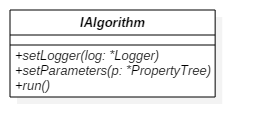
\includegraphics[scale=1, resolution=100]{IAlgorithm}\\
Ein Interface, dass die Funktionen der Algorithmen verallgemeinert und unabhängig von Typen macht, wodurch das Template \hyperref[Workflow:TAlgorithm]{TAlgorithm} polymorph wird.
\beginMembers
\newMemberAbstract{{setLogger}}{*Logger}{void}{Initialisiert einen Logger für den Algorithmus}
\newMemberAbstract{{setParameter}}{*???}{void}{Setze die Parameter für den Algorithmus}
\newMemberAbstract{{run}}{void}{void}{Führe dem Algorithmus auf den dem Plugin bekannten Daten aus.}
\closeMembers

\subsubsection{TAlgorithm}\label{Workflow:TAlgorithm}
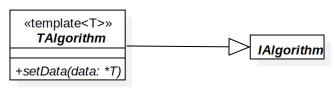
\includegraphics[scale=1, resolution=100]{TAlgorithm}\\
Die Konkrete Implementierung eines Algorithmus.
\beginMembers
\newMemberAbstract{setData}{*T}{void}{Setze die Daten, die der Algorithmus benutzen soll.}
\closeMembers

\subsubsection{EAlgorithmType}
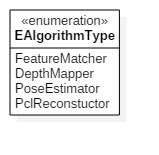
\includegraphics[scale=1, resolution=100]{EAlgorithmType}\\
Eine Klasse, die string-Konstanten enthält, welche den Typ des benutzen \hyperref[Workflow:IAlgorithm]{Algorithmus} in einem \hyperref[Workflow:APlugin]{Plugin} angeben.
\beginAttributes
\newAttribute{FeatureMatcher}{Beschreibt ein Plugin zum Feature Matching.}
\newAttribute{DetphMapper}{Beschreibt ein Plugin zum schätzen von Tiefenkarten.}
\newAttribute{PoseEstimator}{Beschreibt ein Plugin zum schätzen von Posen.}
\newAttribute{PclReconstructor}{beschreibt ein Plugin zur Rekonstruktion von PCL Daten.}
\closeMembers

\subsubsection{AContextDataStore}\label{Workflow:AContextDataStore}
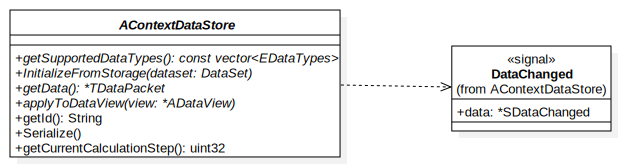
\includegraphics[scale=1, resolution=100]{AContextDataStore}\\
Enthält die Daten, welche für einen Bestimmten \hyperref[Workflow:AWorkflow]{Workflow} zur Verfügung gestellt werden. Jeder Datentyp kann genau einmal im Store vorkommen. Für mehrere gleiche Daten an unterschiedlichen Schritten sind unterschiedliche Klassen anzulegen.
\beginMembers
\newMemberAbstract{getSupportedDataTypes}{void}{const vector<string>}{Gibt eine Liste aller Datentypen in dem Data Store für den Workflow zurück.}
\newMemberAbstract{InitializeFromStorage}{*DataSet}{void}{Initialisiere den Container aus einem Storage heraus.}
\newMemberAbstract{<typename t> getData}{void}{*TDataPacket <t>}{Gibt Daten eines bestimmten Typs zurück, falls vorhanden, null sonst.}
\newMember{getId}{void}{string}{Gibt eine eindeutige ID für den Data Store zurück für Verwaltungszwecke.}
\newMember{Serialize}{void}{void}{Befiehlt dem Data Store, alle Ergebnisse an das DataSet und damit die Festplatte zu übermitteln}
\newMember{getCurrentCalculationStep}{void}{uint32}{Gibt den aktuellen Ausführungsschritt auf diesem Datensatz an.}
\closeMembers
\beginSignals
\newSignal{DataChanged}{*SDataChanged}{Wird aufgerufen, sobald sich Daten geändert haben.}
\closeMembers

\subsubsection{IDataAccess}
Abstrahiert den Zugriff zu den Daten, die von einem bestimmten \hyperref[Workflow:APlugin]{Plugin} benötigt werden und liefert Informationen zu den Verbrauchten und Produzierten Datentypen.
\beginMembers
\newMemberAbstract{bindTo-DataStore}{*AContext-DataStore}{void}{Lade die Daten für den Algorithmus von gegebenem DataStore}
\newMemberAbstract{getInputDataTypes}{void}{const vector<string>}{Eine Liste aller Daten, die als Eingabe benötigt werden.}
\newMemberAbstract{getOutputDataTypes}{void}{const vector<string>}{Eine Liste aller Daten, die als Ausgabe erzeugt werden.}
\closeMembers

\subsubsection{SDataChanged}
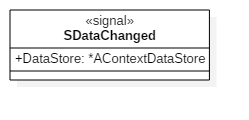
\includegraphics[scale=1, resolution=100]{SDataChanged}\\
Wird gesendet, sobald sich die Daten innerhalb eines \hyperref[Workflow:AContextDataStore]{DataStores} ändern.
\beginAttributes
\newAttribute{DataStore: *AContextDataStore}{Enthält den DataStore, der sich geändert hat}
\closeMembers

\subsubsection{IDataPacket}\label{Workflow:IDataPacket}
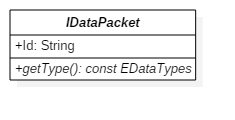
\includegraphics[scale=1, resolution=100]{IDataPacket}\\
Ein Interface, dass dem Template \hyperref[Workflow:TDataPacket]{TDataPacket} Polymorphismus verleiht.
\beginMembers
\newMember{getId}{void}{string}{Gibt die ID des Datenpackets zurück}
\newMember{setId}{string}{void}{Setzt die ID des Datenpackets}
\newMemberAbstract{getType}{void}{const string}{Gibt den Typ der enthaltenen Daten zurück}
\closeMembers

\subsubsection{TDataPacket}\label{Workflow:TDataPacket}
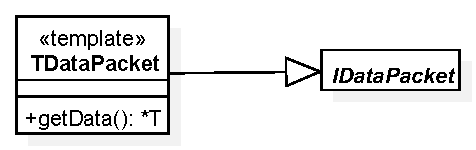
\includegraphics[scale=1, resolution=100]{TDataPacket}\\
Ein Template, dass Zugriff zu einem einzelnen Typ von Daten ermöglicht.
\beginMembers
\newMember{<typename t> getData}{void}{*t}{Gibt die Daten des Packets zurück}
\closeMembers

\subsubsection{EDataTypes}
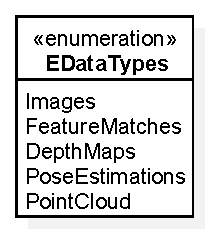
\includegraphics[scale=1,resolution=100]{EDataTypes}\\
Eine Klasse, die string-Konstanten enthält, die den Typ eines Datenpakets definieren.
\beginAttributes
\newAttribute{Images}{Die Eingabebilder}
\newAttribute{FeatureMatches}{Eine Liste an FeatureMatches}
\newAttribute{DepthMaps}{Eine Liste von Tiefenkarten}
\newAttribute{PoseEstimations}{Eine Liste von Posenschätzungen}
\newAttribute{PointCloud}{Ein PointCloud-Datensatz}
\closeMembers

\subsubsection{IDataView} \label{Workflow:IDataView}
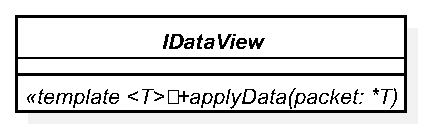
\includegraphics[scale=1,resolution=100]{IDataView}\\
Eine Schnittstelle zum Anwenden der zugrundeliegenden Daten auf die Oberfläche.
\beginMembers
\newMemberAbstract{<typename T> applyData}{*T}{void}{Bekommt ein Datenpacket und wendet dieses dann auf der Oberfläche an.}
\closeMembers

\subsubsection{EExecutionState}
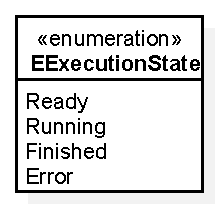
\includegraphics[scale=1,resolution=100]{EExecutionState}\\
Eine Enumeration mit verschiedenen möglichen Ausführungszuständen eines einzelnen Schrittes.
\beginAttributes
\newAttribute{Ready}{Der Schritt ist bereit}
\newAttribute{Running}{Der Schritt wird gerade ausgeführt}
\newAttribute{Finished}{Der Schritt hat die Ausführung beendet}
\newAttribute{Error}{Der Schritt wurde mit einem Fehler beendet}
\closeMembers

\subsubsection{SExecutionStateChanged}
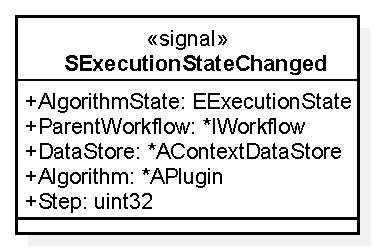
\includegraphics[scale=1,resolution=100]{SExecutionStateChanged}\\
Das Signal wird gesendet, sobald sich der Ausführungszustand eines Datensatzes ändert.
\beginAttributes
\newAttribute{AlgorithmState: EExecutionState}{Der neue Ausführungszustand des Schrittes}
\newAttribute{ParentWorkflow: *AWorkflow}{Der Workflow, der die Meldung gesendet hat}
\newAttribute{DataStore: *AContextDataStore}{Der DataStore, der den neuen Zustand angenommen hat}
\newAttribute{Algorithm: *APlugin}{Der Betroffene Algorithmus}
\newAttribute{Step: uint32}{Der Schritt, in dem sich der DataStore befindet}
\closeMembers

\subsubsection{APlugin}\label{Workflow:APlugin}
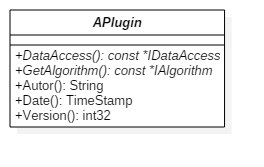
\includegraphics[scale=1,resolution=100]{APlugin}\\
Beschreibt ein einzelnes Plugin, welches einen einzelnen \hyperref[Workflow:IAlgorithm]{Algorithmus} kapselt.
\beginMembers
\newMemberAbstract{DataAccess}{void}{*IDataAccess}{Gibt Zugriff auf eine, für das Plugin passende, implementierung von IDataAccess}
\newMemberAbstract{GetAlgorithm}{void}{*IAlgorithm}{Gibt einen Zugriff auf den Konkreten Algorithmus des Plugins}
\newMember{Autor}{void}{string}{Gibt den Namen des Autors des Plugins zurück}
\newMember{Date}{void}{string}{Gibt das Datum der letzten Änderung an dem Plugincode zurück}
\newMember{Version}{void}{uin32}{Gibt die Version des Plugins zurück}
\closeMembers 

\subsubsection{CPluginManager} \label{Workflow:CPluginManager}
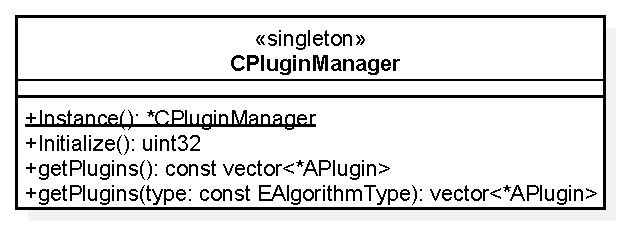
\includegraphics[scale=1,resolution=100]{CPluginManager}\\
Verwaltet alle \hyperref[Workflow:APlugin]{Plugins}, die vom System gefunden wurden.
\beginMembers
\newMemberStatic{Instance}{void}{*CPluginManager}{Gibt die Instanz des Plugin Managers zurück}
\newMember{Initialize}{void}{int32}{Initialisiert den Manager und lädt alle Plugins. Liefert einen Standard Returncode.}
\newMember{getPlugins}{void}{const vector<*APlugin>}{Gibt eine Liste aller Plugins zurück}
\newMember{getPlugins}{const string}{vector <*APlugin>}{Gibt einer Liste aller Plugins von einem gegebenen Typ zurück.}
\closeMembers

\subsubsection{AWorkflow}\label{Workflow:AWorkflow}
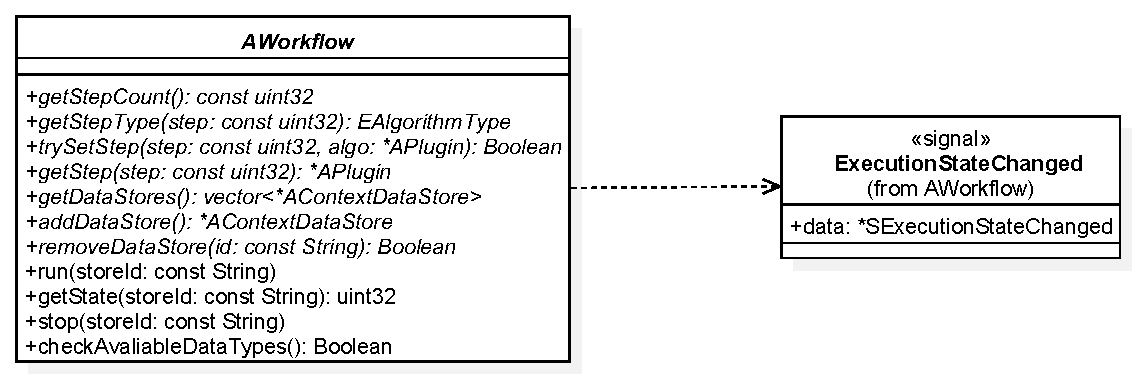
\includegraphics[scale=1,resolution=100]{AWorkflow}\\
Verwaltet \hyperref[Workflow:IAlgorithm]{Algorithmen} und \hyperref[Workflow:AContextDataStore]{Daten}, die für eine bestimmte Problemstellung und Herangehensweise benötigt werden.
\beginMembers
\newMemberAbstract{getStepCount}{void}{const uint32}{Gibt die Anzahl der Schritte im Workflow zurück}
\newMemberAbstract{getStepType}{const uint32}{string}{Gibt den Typ eines Algorithmus für einen bestimmten Schritt zurück}
\newMemberAbstract{trySetStep}{const uint32, *APlugin}{bool}{Versucht, ein Plugin einem Schritt zuzuweisen. True, wenn das Plugin kompatibel war.}
\newMemberAbstract{getStep}{const uint32}{*APlugin}{Liefert das gesetzte Plugin für einen bestimmten Schritt}
\newMemberAbstract{getDataStores}{void}{vector<*AContextDataStore>}{Liefert alle registrierten DataStores für diesen Workflow}
\newMemberAbstract{addDataStore}{void}{*AContextDataStore}{Gibt eine Instanz eines DataStores für diesen Workflow zurück und fügt ihn in die Verwaltung ein.}
\newMemberAbstract{removeDataStore}{const string}{void}{Entfernt einen DataStore anhand seiner ID}
\newMember{run}{const string}{void}{Startet die Ausführung eines bestimmten DataStores}
\newMember{getState}{const string}{uin3232}{Gibt den aktuellen Schritt eines DataStores an, -1 für ende, < -10 für Fehler bei schritt -n-10}
\newMember{checkAvailableDataTypes}{void}{bool}{Prüft, ob die Algorithmen alle benötigten Daten auch produzieren}
\closeMembers
\beginSignals
\newSignal{ExecutionStateChanged}{*SExecutionStateChanged}{Wird aufgerufen, sobald sich der Ausführungszustand eines Algorithmus ändert.}
\closeMembers

\subsection{Konkrete Umsetzungen}
Hier werden Implementierungen der oben genannten Konstrukte nach den Forderungen im Pflichtenheft exemplarisch für jeweils eine Implementierung pro Klasse gezeigt, da sich einiges Wiederholt und keinen Mehrwert bieten kann, vor allem da das Programm in diese Richtungen erweiterbar ist.
\subsubsection{CFourPhaseWorkflow} \label{Workflow:CFourPhaseWorkflow}
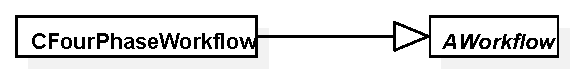
\includegraphics[scale=1,resolution=100]{CFourPhaseWorkflow}\\
Implementiert \hyperref[Workflow:AWorkflow]{AWorkflow} und stellt einen vier Phasen Workflow zur Verfügung, der das einstellen von vier Algorithmen erlaubt.
\subsubsection{CFourPhaseWorkflowDataStore}
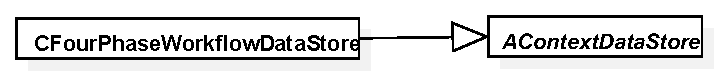
\includegraphics[scale=1, resolution=100]{CFourPhaseWorkflowDataStore}\\
Stellt den Datenspeicher für den \hyperref[Workflow:CFourPhaseWorkflow]{vier Phasen Workflow} bereit.
\subsubsection{CStereoRectificationPlugin}
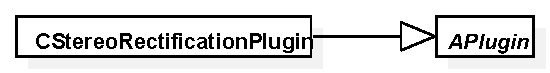
\includegraphics[scale=1,resolution=100]{CStereoRectificationPlugin}\\
Ein Beispiel Plugin für den Algorithmus Stereo Rectification.
\subsubsection{CStereoRectificationData}
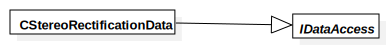
\includegraphics[scale=1,resolution=100]{CStereoRectificationData}\\
Ein Datenadapter für den Algorithmus Stereo Rectification
\subsubsection{CStereoRectificationAlgorithm}
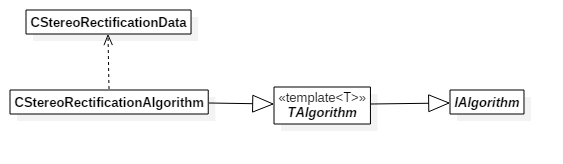
\includegraphics[scale=1,resolution=100]{CStereoRectificationAlgorithm}\\
Die Konkrete Implementierung des Stereo Rectification Algorithmus.

\section{Pakete}
%Einteilung der Teilmodule in Pakete 
Das Modul Workflow kann in zwei größere Pakete eingeteilt werden.
\subsection{Plugin}
Das Paket Plugin beinhaltet alle Klassen, die in eine Bibliothek ausgelagert werden und mit \hyperref[Workflow:APlugin]{APlugin} zusammenhängen.
\\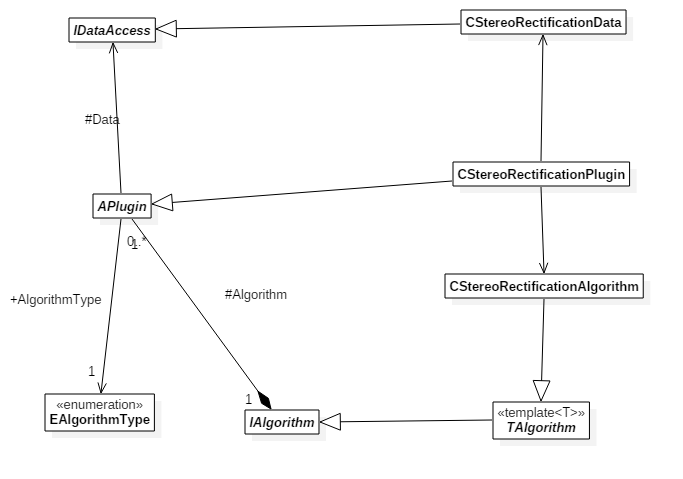
\includegraphics[scale=1,resolution=100]{PluginSimple}
%Bild des Pakets mit vereinfachter Klassendarstellung
%Begründung / Dokumentation / Erklärung zum Paket
\subsection{Workflow}
Das Paket Workflow enthält Klassen, die für einen einzelnen Workflow nötig sind und später eventuell auch ausgelagert werden können.
\\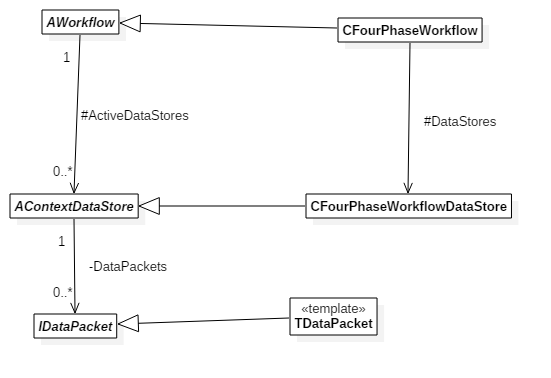
\includegraphics[scale=1,resolution=100]{WorkflowSimple}
\section{Entwurfsmuster}
% verwendete Entwurfsmuster aufzählen erklären etc mit verinfachtem Diagramm (Klassen ohne Inhalt nur die Namen)
\begin{itemize}
	\item \textbf{Singleton}
	\\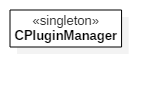
\includegraphics[scale=1, resolution=100]{SingletonPattern}
	\\ Der \hyperref[Workflow:CPluginManager]{Plugin Manager} benutzt dieses Pattern, damit Plugins nicht mehrmals geladen werden können, was zu Zugriffsfehlern führen kann.
	\item \textbf{Visitor Pattern}
	\\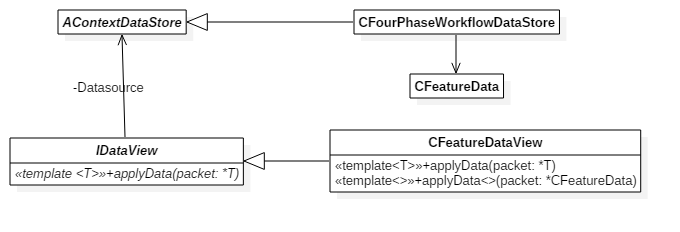
\includegraphics[scale=1,resolution=120]{VisitorPattern}
	\\ Das \hyperref[Workflow:IDataView]{DataView} benutzt das Visitorpattern, um Downcasts von Datenpacketen zu vermeiden.
	\item \textbf{Factory Pattern}
	\\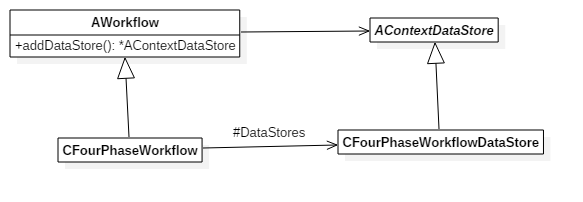
\includegraphics[scale=1,resolution=100]{FactoryPattern}
	\\ Alle Referenzen zu \hyperref[Workflow:IDataAccess]{IDataAccess} und \hyperref[Workflow:AContextDataStore]{AContextDataStore} werden über das Factory Pattern innerhalb des Behälters erzeugt.
	\item \textbf{Bridge Pattern}
	\\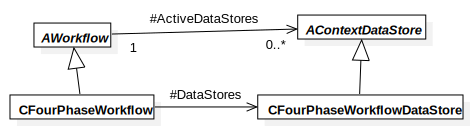
\includegraphics[scale=1, resolution=100]{BridgePattern}
	\\ Das Bridge Pattern wird durchgängig bei den allermeisten Klassen im Workflow angewendet. Ausnahmen sind \hyperref[Workflow:CPluginManager]{CPluginManager} und \hyperref[Workflow:IDataView]{IDataView}.
	\item \textbf{Adapter Pattern}
	\\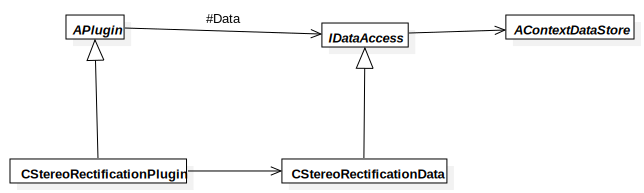
\includegraphics[scale=1, resolution=100]{AdapterPattern}
	\\ Das Adapter Pattern wird bei \hyperref[Workflow:IDataAccess]{IDataAccess} und den spezifischen Implementierungen in den Algorithmen angewendet, damit die Algorithmen von dem Datenzugriff entkoppelt werden.
	\item \textbf{Observer Pattern}
	\\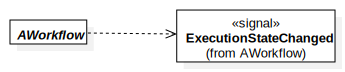
\includegraphics[scale=1, resolution=100]{ObserverPattern}
	\\ Die Qt-Signale in den Klassen \hyperref[Workflow:AWorkflow]{AWorkflow} und \hyperref[Workflow:AContextDataStore]{AContextDataStore} implmentieren das Observer Pattern.
\end{itemize}
\section{Klassendiagramm}
\subsection{Übersicht}
% Klassendiagramm des Moduls
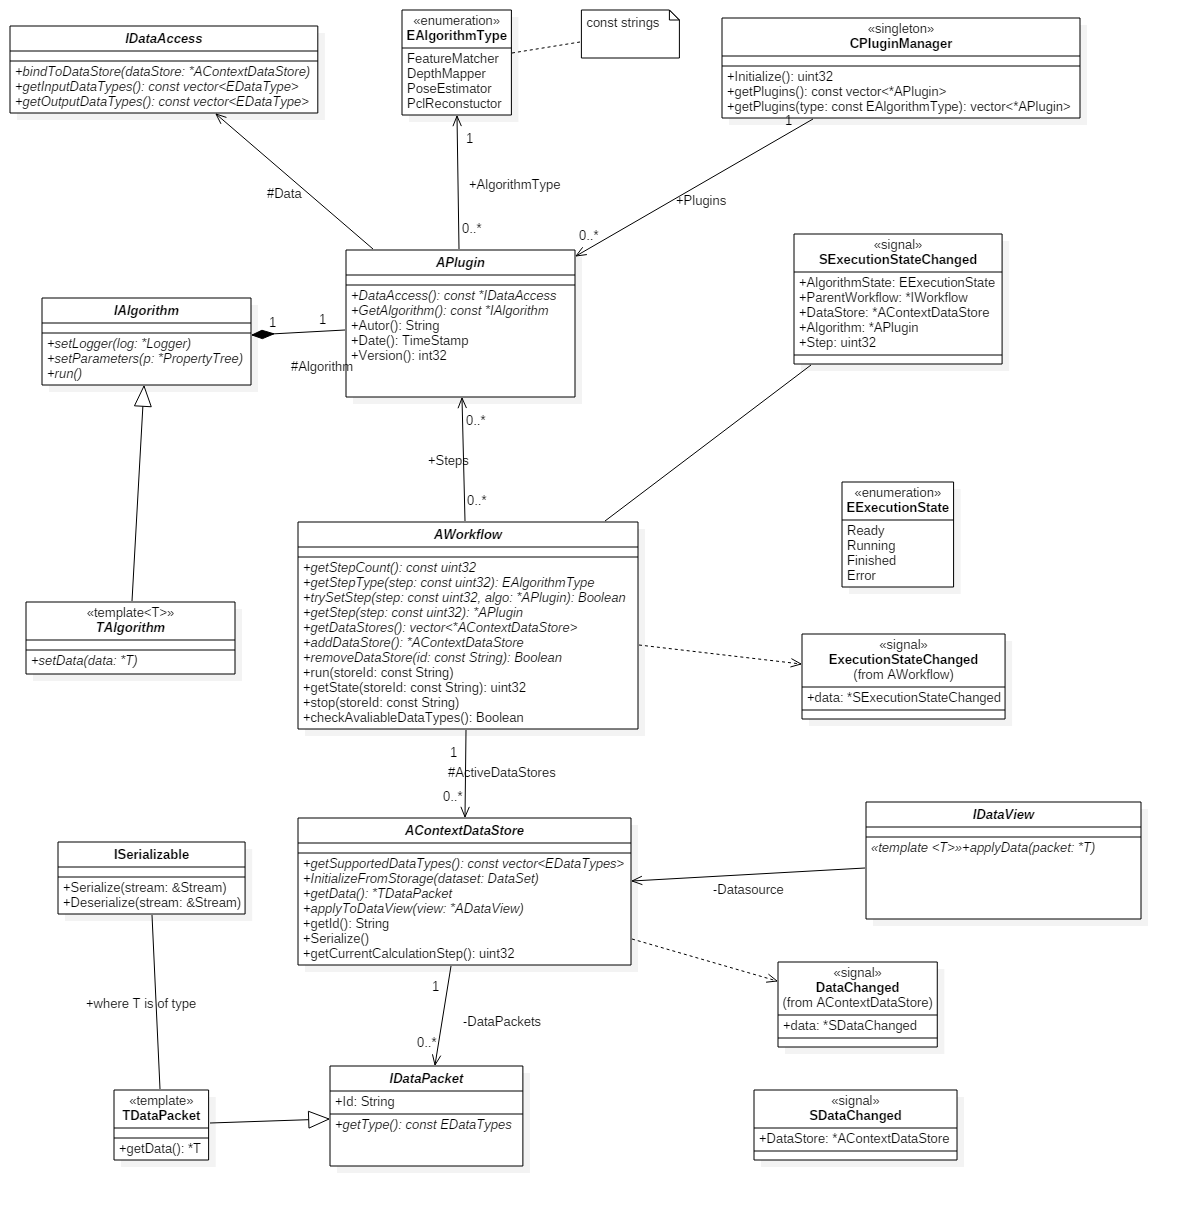
\includegraphics[width=\linewidth]{overview.png}
\subsection{Beispiel: Plugin}
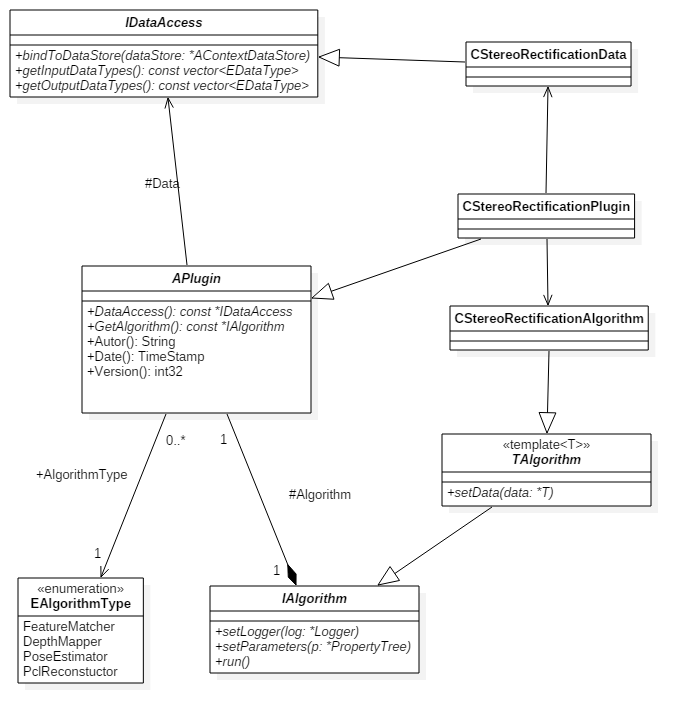
\includegraphics[width=\linewidth]{Plugin.png}
\subsection{Beispiel: Workflow}
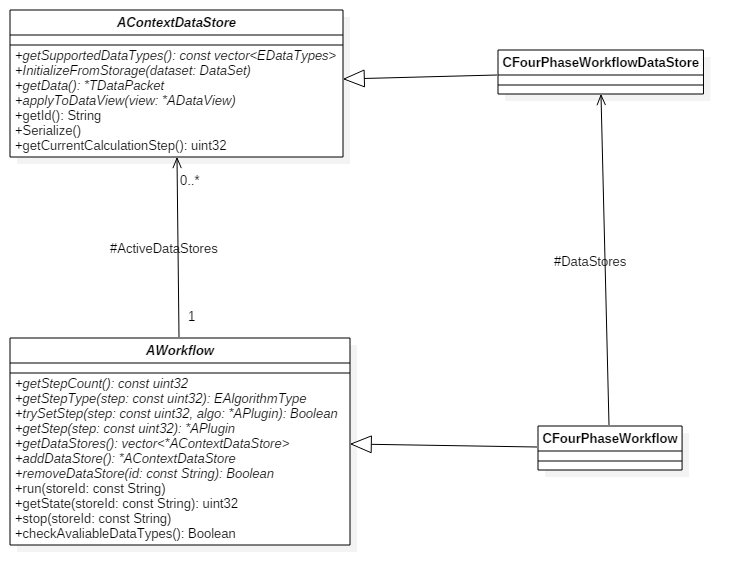
\includegraphics[width=\linewidth]{Workflow.png}